\documentclass{article}
\title{Homework1}
\author{Blue}
\date{20230118}
\usepackage{geometry}
\geometry{a4paper,scale=0.8}
\usepackage{graphicx}
\usepackage{float}
\usepackage{indentfirst}
\usepackage[namelimits]{amsmath} %数学公式
\usepackage{amssymb}             %数学公式
\usepackage{color}
\usepackage{longtable}
\usepackage{listings}
\lstset{
language=Matlab,
numbers=left,
keywordstyle=\color{blue},
numberstyle=\tiny,
breaklines=true,
extendedchars=flase
}

\begin{document}
\pagenumbering{gobble}
\maketitle

\section{Plotting in Matlab}
\noindent(i)
\begin{figure}[H]
\centering
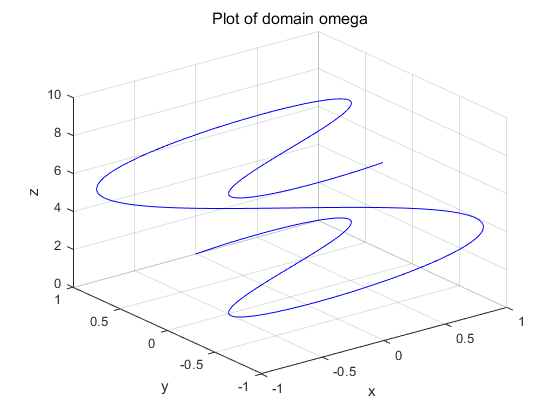
\includegraphics{plot.png}
\caption{3D curve}
\end{figure}
\noindent (ii)result:17.222032186553953\par
code:\par
func=@(x)((2*cos(2*x)).\^{}2+(-sin(x)).\^{}2+1).\^{}0.5;\par
integral(func,0,3*pi)\par


\section{Floating-Point Exceptions}
\begin{itemize}
\item code:single(exp(500))\quad get:\quad {\underline{\textcolor{blue}{single}}} Inf\\
code:exp(1000) \quad get: Inf\quad(This is in double form)

\item code:1/0 \quad get:\quad Inf \quad The answer makes sense to me.\\
code:Inf/-Inf \quad get:\quad NaN\\
code:0/0 \quad get:\quad NaN

\item code:\quad exp(100)<Inf \quad get:\quad {\underline{\textcolor{blue}{logical}}} 1\\
code:\quad -exp(100)>-Inf \quad get:\quad {\underline{\textcolor{blue}{logical}}} 1\\
code:\quad exp(100)<NaN \quad get:\quad {\underline{\textcolor{blue}{logical}}} 0\\
code:\quad exp(100)>NaN \quad get:\quad {\underline{\textcolor{blue}{logical}}} 0\\
code:\quad exp(100)==NaN \quad get:\quad {\underline{\textcolor{blue}{logical}}} 0\\
code:\quad Inf==NaN \quad get:\quad {\underline{\textcolor{blue}{logical}}} 0\\
code:\quad Inf>NaN \quad get:\quad {\underline{\textcolor{blue}{logical}}} 0\\
code:\quad Inf<NaN \quad get:\quad {\underline{\textcolor{blue}{logical}}} 0\\
code:\quad Inf==-NaN \quad get:\quad {\underline{\textcolor{blue}{logical}}} 0\\
code:\quad Inf>-NaN \quad get:\quad {\underline{\textcolor{blue}{logical}}} 0\\
code:\quad Inf<-NaN \quad get:\quad {\underline{\textcolor{blue}{logical}}} 0\\
conclusion:-Inf<normal number<Inf. Comparison between NaN and normal number or Infs get nothing.
\item code:x=0/0 \quad get:\quad x=NaN\\
code:x+100 \quad get:\quad x=NaN\\
code:x-100 \quad get:\quad x=NaN\\
code:x*100 \quad get:\quad x=NaN\\
code:x/100 \quad get:\quad x=NaN\\
code:x/0 \quad get:\quad x=NaN\\
code:x*0 \quad get:\quad x=NaN
\item code:x=1/exp(500); sqrt(x) \quad get:\quad x=2.669190215541276e-109\\
code:x=1/(-exp(500)); sqrt(x) \quad get:\quad x=0.000000000000000e+00 +2.669190215541276e-109i\\
code:x=1/exp(750); sqrt(x) \quad get:\quad x=0\\
code:x=1/(-exp(750)); sqrt(x) \quad get:\quad x=0\\
code:sqrt(+0) \quad get:\quad 0\\
code:sqrt(-0) \quad get:\quad 0\\
There is difference between +0 and -0 in MATLAB. The following code shows the difference.\\
code:1/(+0) \quad get:\quad x=Inf\\
code:1/(-0) \quad get:\quad x=-Inf
\end{itemize}



\section{Algorithm to Compute $\pi$}
3.1 Using the absolute error we get the following format.
\begin{center}
\begin{longtable}{|c|c|c|c|c|}
Iteration	&	Single precision	&	Double precision	&	Single error	&	Double error	\\ \hline
1	&	0.5773503	&	0.577350269	&	2.5642424	&	2.564242384	\\ \hline
2	&	3.21539	&	3.215390309	&	0.0737973	&	0.073797656	\\ \hline
3	&	3.1596599	&	3.159659942	&	0.0180672	&	0.018067289	\\ \hline
4	&	3.1460876	&	3.146086215	&	0.004495	&	0.004493562	\\ \hline
5	&	3.1426797	&	3.1427146	&	0.001087	&	0.001121946	\\ \hline
6	&	3.1420677	&	3.14187305	&	0.000475	&	0.000280396	\\ \hline
7	&	3.1412809	&	3.141662747	&	0.0003118	&	7.00935E-05	\\ \hline
8	&	3.1336737	&	3.141610177	&	0.007919	&	1.7523E-05	\\ \hline
9	&	3.1412809	&	3.141597034	&	0.0003118	&	4.38073E-06	\\ \hline
10	&	3.0441403	&	3.141593749	&	0.0974523	&	1.09523E-06	\\ \hline
11	&	2.9564998	&	3.141592928	&	0.1850928	&	2.74284E-07	\\ \hline
12	&	3.0441403	&	3.141592726	&	0.0974523	&	7.20328E-08	\\ \hline
13	&	0	&	3.141592672	&	3.1415927	&	1.81518E-08	\\ \hline
14	&	NaN	&	3.141592619	&	NaN	&	3.46889E-08	\\ \hline
15	&	NaN	&	3.141592672	&	NaN	&	1.81518E-08	\\ \hline
16	&	NaN	&	3.141591936	&	NaN	&	7.17708E-07	\\ \hline
17	&	NaN	&	3.141592672	&	NaN	&	1.81518E-08	\\ \hline
18	&	NaN	&	3.141581008	&	NaN	&	1.1646E-05	\\ \hline
19	&	NaN	&	3.141592672	&	NaN	&	1.81518E-08	\\ \hline
20	&	NaN	&	3.141406155	&	NaN	&	0.000186499	\\ \hline
21	&	NaN	&	3.140543492	&	NaN	&	0.001049161	\\ \hline
22	&	NaN	&	3.140006865	&	NaN	&	0.001585789	\\ \hline
23	&	NaN	&	3.134945376	&	NaN	&	0.006647278	\\ \hline
24	&	NaN	&	3.140006865	&	NaN	&	0.001585789	\\ \hline
25	&	NaN	&	3.224515244	&	NaN	&	0.08292259	\\ \hline
26	&	NaN	&	2.791117213	&	NaN	&	0.350475441	\\ \hline
27	&	NaN	&	0	&	NaN	&	3.141592654	\\ \hline
28	&	NaN	&	NaN	&	NaN	&	NaN	\\ \hline
29	&	NaN	&	NaN	&	NaN	&	NaN	\\ \hline
30	&	NaN	&	NaN	&	NaN	&	NaN	\\ \hline



\end{longtable}
\end{center}
\begin{figure}[H]
\centering
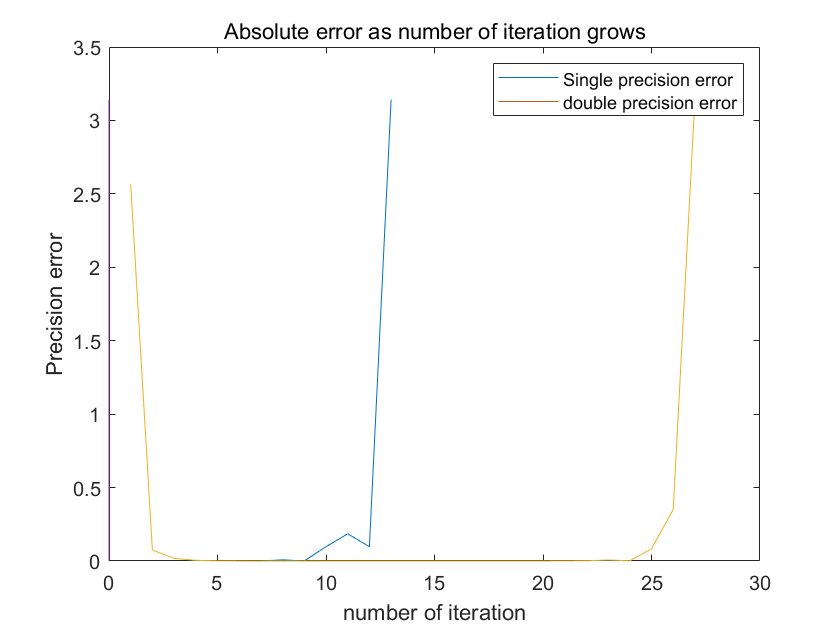
\includegraphics[width=0.4\textwidth,height=0.3\textwidth]{precision.png}
\caption{Single precision and double precision}
\end{figure}
According to the format above, at the beginning, the round-off error is not large. As the loop runs, $t_{i}$ becomes smaller and smaller.When i=10 for single precision, and i=19 for double precision, the round-off error is large enough to be the main part of the error. And the estimation becomes less accurate. When $t_{i}$ becomes so close to 0 that due to round-off error the numerator is 0 at calculation, the answer is 0. That is when i=13 for single precision and i=27 for double precision.\\
At first the loop doesn't calculate enought times, it may be can be called as a kind of truncation error. Later when the i becomes large enought that the answer approximate the limitation of the round-off systems. The round-off error becomes the dominant error. Each time the loop goes, the round-off error accumulate, and finally the answer becomes 0 and NOT A NUMBER.\par
~\\
3.2
Rewrite the equation into the following form:
\begin{equation}
\begin{split}
t_{i+1}&=\frac{\sqrt{1+t_{i}^{2}}-1}{t_{i}}\times\frac{1+\sqrt{1+t_{i}^{2}}}{1+\sqrt{1+t_{i}^{2}}}\\
&=\frac{t_{i}^{2}}{t_{i}\left(1+\sqrt{1+t_{i}^{2}}\right)}\\
&=\frac{t_{i}}{1+\sqrt{1+t_{i}^{2}}}.
\end{split}
\end{equation}
Using the new form, we get the following format:
\begin{center}
\begin{longtable}{|c|c|c|c|c|}
Iteration	&	Single precision	&	Double precision	&	Single error	&	Double error	\\ \hline
1	&	0.5773503	&	0.577350269	&	2.5642424	&	2.564242384	\\ \hline
2	&	3.2153902	&	3.215390309	&	0.0737976	&	0.073797656	\\ \hline
3	&	3.1596601	&	3.159659942	&	0.0180674	&	0.018067289	\\ \hline
4	&	3.1460867	&	3.146086215	&	0.004494	&	0.004493562	\\ \hline
5	&	3.142715	&	3.1427146	&	0.0011223	&	0.001121946	\\ \hline
6	&	3.1418734	&	3.14187305	&	0.0002807	&	0.000280396	\\ \hline
7	&	3.1416628	&	3.141662747	&	0.0000702	&	7.00935E-05	\\ \hline
8	&	3.1416101	&	3.141610177	&	0.0000175	&	1.7523E-05	\\ \hline
9	&	3.141597	&	3.141597034	&	0.0000044	&	4.38073E-06	\\ \hline
10	&	3.1415942	&	3.141593749	&	0.0000015	&	1.09518E-06	\\ \hline
11	&	3.1415935	&	3.141592927	&	0.0000008	&	2.73795E-07	\\ \hline
12	&	3.1415935	&	3.141592722	&	0.0000008	&	6.84488E-08	\\ \hline
13	&	3.1415935	&	3.141592671	&	0.0000008	&	1.71122E-08	\\ \hline
14	&	3.1415935	&	3.141592658	&	0.0000008	&	4.27805E-09	\\ \hline
15	&	3.1415935	&	3.141592655	&	0.0000008	&	1.06952E-09	\\ \hline
16	&	3.1415935	&	3.141592654	&	0.0000008	&	2.67381E-10	\\ \hline
17	&	3.1415935	&	3.141592654	&	0.0000008	&	6.6847E-11	\\ \hline
18	&	3.1415935	&	3.141592654	&	0.0000008	&	1.6714E-11	\\ \hline
19	&	3.1415935	&	3.141592654	&	0.0000008	&	4.181E-12	\\ \hline
20	&	3.1415935	&	3.141592654	&	0.0000008	&	1.047E-12	\\ \hline
21	&	3.1415935	&	3.141592654	&	0.0000008	&	2.64E-13	\\ \hline
22	&	3.1415935	&	3.141592654	&	0.0000008	&	6.8E-14	\\ \hline
23	&	3.1415935	&	3.141592654	&	0.0000008	&	2E-14	\\ \hline
24	&	3.1415935	&	3.141592654	&	0.0000008	&	7E-15	\\ \hline
25	&	3.1415935	&	3.141592654	&	0.0000008	&	4E-15	\\ \hline
26	&	3.1415935	&	3.141592654	&	0.0000008	&	4E-15	\\ \hline
27	&	3.1415935	&	3.141592654	&	0.0000008	&	4E-15	\\ \hline
28	&	3.1415935	&	3.141592654	&	0.0000008	&	4E-15	\\ \hline
29	&	3.1415935	&	3.141592654	&	0.0000008	&	4E-15	\\ \hline
30	&	3.1415935	&	3.141592654	&	0.0000008	&	4E-15	\\ \hline
\end{longtable}
\end{center}
\begin{figure}[H]
\centering
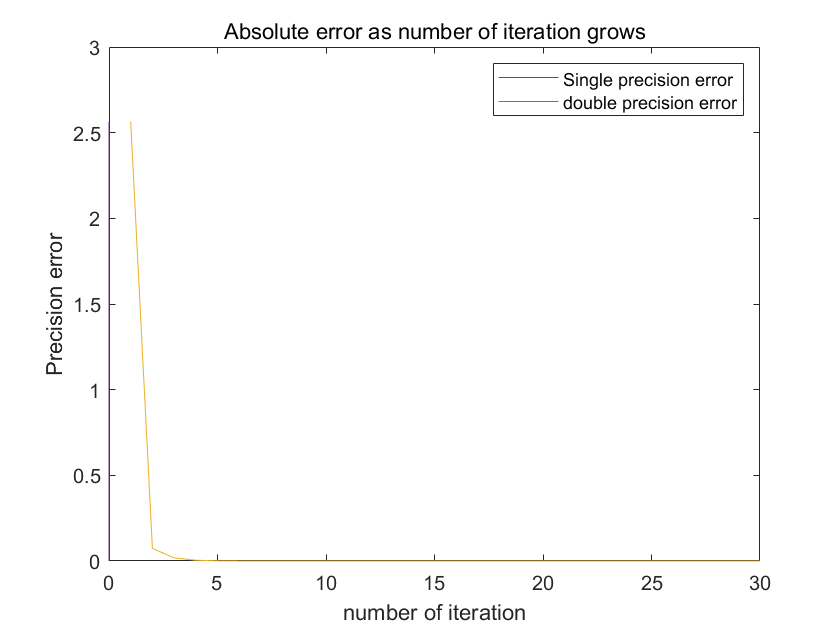
\includegraphics[width=0.4\textwidth,height=0.3\textwidth]{precision1.png}
\caption{Single precision and double precision}
\end{figure}
As the format shows, the figure is accurate to 6 decimal places using the single precision. The figure is accurate to 14 decimal places using the double precision. Its accuracy improves a lot.






\section{Round Off vs Truncation Error}
\begin{center}
\begin{longtable}{|c|c|c|c|c|}
Iteration	&	Single precision	&	Double precision	&	Single error	&	Double error	\\ \hline
1	&	-0.6924973	&	-0.692497605	&	0.0146095	&	0.014609176	\\ \hline
2	&	-0.7034302	&	-0.703431597	&	0.0036766	&	0.003675184	\\ \hline
3	&	-0.7061806	&	-0.706186549	&	0.0009262	&	0.000920233	\\ \hline
4	&	-0.7068634	&	-0.706876633	&	0.0002434	&	0.000230148	\\ \hline
5	&	-0.7070313	&	-0.707049239	&	0.0000755	&	5.75426E-05	\\ \hline
6	&	-0.7067871	&	-0.707092395	&	0.0003197	&	1.4386E-05	\\ \hline
7	&	-0.7070313	&	-0.707103185	&	0.0000755	&	3.59652E-06	\\ \hline
8	&	-0.703125	&	-0.707105882	&	0.0039818	&	8.99135E-07	\\ \hline
9	&	-0.6875	&	-0.707106556	&	0.0196068	&	2.24792E-07	\\ \hline
10	&	-0.6875	&	-0.707106725	&	0.0196068	&	5.63394E-08	\\ \hline



\end{longtable}
\end{center}
\begin{figure}[H]
\centering
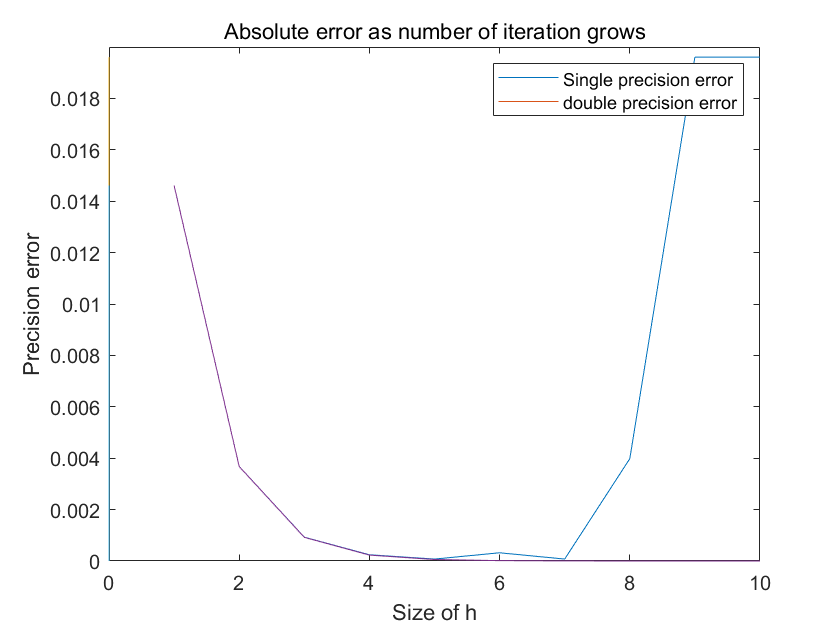
\includegraphics[width=0.4\textwidth,height=0.3\textwidth]{problem4.png}
\caption{Absolute error as size of h grows}
\end{figure}

Comparing to the known derivative, which is $-sin\left(\frac{\pi}{4}\right)=-\frac{\sqrt{2}}{2}$, we get the format above.\\
For single precision, due to round off error, we get the most accurate answer at 5 and 7.\\
For double precision, we get the most accurate answer at more than 10.



\section{ Well- or Ill-conditioned?}
Let $y=sin(x)$, then $\frac{dy}{dx}=cos(x)$
\begin{equation}
\begin{split}
\kappa &=\sup_{\delta x\neq 0}\frac{||\delta y||/||y||}{||\delta x||/||x||} \\
&=\sup_{\delta x\neq 0}\frac{\frac{||\delta y||}{||\delta x||}}{|y|/|x|}\\
&=\frac{\lim\limits_{\delta x\to 0}\frac{||\delta y||}{||\delta x||}}{|y|/|x|}\\
&=\frac{y'(x)}{|y|/|x|}.
\end{split}
\end{equation}
When x near 0, we get 
\begin{equation}
\lim_{x \to 0}\frac{sin(x)}{x}=1
\end{equation}
So 
\begin{equation}
\begin{split}
\kappa_{x \to 0}&=\lim_{x \to 0}\frac{cos(x)}{|sin(x)|/|x|}\\
&=\frac{\lim\limits_{x \to 0}cos(x)}{\lim\limits_{x \to 0}\frac{|sin(x)|}{|x|}}\\
&=1.
\end{split}
\end{equation}
So sin(x) is well-conditioned when x near 0.\\
 However, when x near $2\pi$. $y'(x)\to 1$, $sin(x)\to 0$, so
\begin{equation}
\begin{split}
\kappa_{x \to 2\pi}&=\lim_{x \to 2\pi}\frac{cos(x)}{|sin(x)|/|x|}\\
&=+\infty.
\end{split}
\end{equation}
Therefore, when x near $2\pi$ sin(x) is ill-conditioned.




\section{Code}

\subsection{Plotting in Matlab}
\begin{lstlisting}
t=0:0.01:3*pi;
x=sin(2*t);
y=cos(t);
z=t;
plot3(x,y,z,'blue-')
grid on;
xlabel('x');
ylabel('y');
zlabel('z');
title('Plot of domain omega','FontSize',12)
func=@(x)((2*cos(2*x)).^2+(-sin(x)).^2+1).^0.5;
integral(func,0,3*pi)
\end{lstlisting}
\subsection{Floating-Point Exceptions}
The code is presented in the answer.
\subsection{Algorithm to Compute $\pi$}
\paragraph{The original code}
\begin{lstlisting}
Sp=zeros(30,1,'single');
Dp=zeros(30,1);
Spe=zeros(30,1,'single');
Dpe=zeros(30,1);
ts=single(1/(sqrt(3)));
td=1/sqrt(3);
Sp(1)=ts;
Spe(1)=abs(single(pi)-ts);
Dp(1)=td;
Dpe(1)=abs(pi-td);
for i=2:30
    ts=(calt(ts));
    Sp(i)=ts*6*(2^(i-1));
    Spe(i)=abs((pi)-ts*6*(2^(i-1)));
    td=calt(td);
    Dp(i)=td*6*(2^(i-1));
    Dpe(i)=abs(pi-td*6*(2^(i-1)));
end
Sp
Spe
Dp
Dpe
x=zeros(30);
for i=1:30
    x(i)=i;
end
plot(x,Spe,x,Dpe)
title('Absolute error as number of iteration grows')
ylabel('Precision error')
xlabel('number of iteration')
legend('Single precision error','double precision error')


function x=calt(t)
x=(sqrt(1+t^2)-1)/t;
end
\end{lstlisting}

\subsubsection{The improved code}

\begin{lstlisting}
Sp=zeros(30,1,'single');
Dp=zeros(30,1);
Spe=zeros(30,1,'single');
Dpe=zeros(30,1);
ts=single(1/(sqrt(3)));
td=1/sqrt(3);
Sp(1)=ts;
Spe(1)=abs(single(pi)-ts);
Dp(1)=td;
Dpe(1)=abs(pi-td);
for i=2:30
    ts=(calt(ts));
    Sp(i)=ts*6*(2^(i-1));
    Spe(i)=abs((pi)-ts*6*(2^(i-1)));
    td=calt(td);
    Dp(i)=td*6*(2^(i-1));
    Dpe(i)=abs(pi-td*6*(2^(i-1)));
end
Sp
Spe
Dp
Dpe
x=zeros(30);
for i=1:30
    x(i)=i;
end
plot(x,Spe,x,Dpe)
title('Absolute error as number of iteration grows')
ylabel('Precision error')
xlabel('number of iteration')
legend('Single precision error','double precision error')
function x=calt(t)
x=t/(sqrt(t^2+1)+1);
end
\end{lstlisting}
\subsection{Round off vs Truncation Error}
\begin{lstlisting}
Sp=zeros(30,1,'single');
Dp=zeros(30,1);
Spe=zeros(30,1,'single');
Dpe=zeros(30,1);
ts=single(1/(sqrt(3)));
td=1/sqrt(3);
Sp(1)=ts;
Spe(1)=abs(single(pi)-ts);
Dp(1)=td;
Dpe(1)=abs(pi-td);
for i=2:30
    ts=(calt(ts));
    Sp(i)=ts*6*(2^(i-1));
    Spe(i)=abs((pi)-ts*6*(2^(i-1)));
    td=calt(td);
    Dp(i)=td*6*(2^(i-1));
    Dpe(i)=abs(pi-td*6*(2^(i-1)));
end
Sp
Spe
Dp
Dpe
x=zeros(30);
for i=1:30
    x(i)=i;
end
plot(x,Spe,x,Dpe)
title('Absolute error as number of iteration grows')
ylabel('Precision error')
xlabel('number of iteration')
legend('Single precision error','double precision error')


function x=calt(t)
x=(sqrt(1+t^2)-1)/t;
end
\end{lstlisting}
\end{document}

